\documentclass[slidestop,compress,mathserif,xcolor=svgnames,table]{beamer}

\usepackage[spanish]{babel}
\usepackage[latin1]{inputenc} % Ambos para soluci�n de asuntos de idioma.
\usepackage{amsmath, amsfonts, amssymb} % Matem�ticas varias.
\usepackage{longtable} % Tabla larga necesaria para el ap�ndice de simbolog�a.
%\usepackage{multimedia}
\usepackage{movie15}
\usepackage{enumitem}
\usepackage{wrapfig}
\usepackage{float}
\setitemize{leftmargin=*}

\setitemize[1]{label=\tiny$\blacksquare$}
\setitemize[2]{label=\tiny$\bullet$}
\setitemize[3]{label=\tiny$\bullet$}

% --- Arreglos varios para la inclusion de im�genes
\usepackage{subfigure}
\DeclareGraphicsExtensions{.png,.jpg,.pdf,.mps,.gif,.bmp}

% ================= CONFIGURACI�N DEL BEAMER ====================
% ===============================================================
\mode<presentation>{
% \usepackage{beamerthemeclassic}
% \setbeameroption{show notes}
% \setbeameroption{hide notes}
\setbeameroption{notes on second screen}
\setbeamercovered{transparent}
% \usetheme{Warsaw}
\usetheme{Frankfurt}
% \usetheme{Berlin}
% \usetheme{Madrid}
% \usetheme{Antibes}
% \usecolortheme{rose}
% \usecolortheme{lily} % Beamer color theme
% \usecolortheme{seahorse}
% \usecolortheme{fly}
% \usecolortheme[RGB={70,110,45}]{structure}	%verde primaveral
\usecolortheme[RGB={100,12,20}]{structure}	%rojo sangre
% \usecolortheme[RGB={30,40,30}]{structure}	% Luto
% \usecolortheme[RGB={160,230,70}]{structure}	%verde manzana Grand-Smith
\usefonttheme[onlymath]{serif}
\usefonttheme{professionalfonts}
\setbeamerfont{frametitle}{family=\rmfamily,shape=\scshape,size=\normalsize}
\setbeamertemplate{frametitle}[default][center]
}
% Make a TOC appear before every section
%\AtBeginSection[]
%{\begin{frame}
%  \tableofcontents[currentsection]
% \end{frame}
%}
%\AtBeginNote{Notas:\par}


% ========================= COMANDOS ============================
% ===============================================================
\newcommand{\ket}[1]{|#1\rangle}
\newcommand{\bcol}{\begin{columns}[T]}
\newcommand{\ecol}{\end{columns}}
\newcommand{\col}[1][0.5]{\column{#1\textwidth}}
\newenvironment{itemize*}%
  {\begin{itemize}%
    \setlength{\topsep}{10pt}%
    \setlength{\itemsep}{0pt}%
    \setlength{\parskip}{10pt}}%
  {\end{itemize}
}

% =================== DATOS DEL DOCUMENTO =======================
% ===============================================================
\author{Manuel L�pez, Santiago Paternain, Rodrigo Rosa, Mat�as Tailani�n}
\date{19 de Setiembre de 2011}
\title{\textit{Implementaci�n de un UAV con arquitectura de Quadcopter}}
\subtitle{Segundo Hito}



% ===============================================================
% ===============================================================
% ================ COMIENZO DEL DOCUMENTO =======================
% ===============================================================
% ===============================================================



\begin{document}

% ========================= FRAME ===============================
% ===============================================================
\frame[plain]{
  \titlepage
}

\section{Panorama Global}
\begin{frame}
\frametitle{Panorama Global}

Dise�ar e integrar un \textbf{sistema de control} que permita el vuelo \emph{aut�nomo} de un Cuadric�petro comercial.
\pause

\begin{columns}

\column{2.2in}

\begin{figure}[h!]
  \begin{center}
  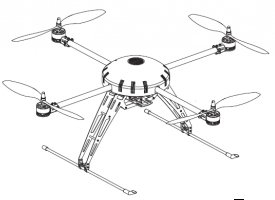
\includegraphics[width=.85\textwidth]{./Pics/quad.jpg}
  \end{center}
\end{figure}

\column{2.2in}

\begin{itemize}
	\item Generador de rutas\pause
	\item Instrumentaci�n: obtener variables del sistema \pause
	\item Actuador sobre motores
\end{itemize}

\end{columns}
\pause
\vspace{15pt}
No se dise�ar� ni la mec�nica ni la electr�nica del sistema.\\
Se integrar�n los componentes.\\
Se conservar� la posibilidad del manejo manual

\end{frame}

\section{Planificaci�n Original}
% ========================= FRAME ===============================
% ===============================================================
\begin{frame}
\frametitle{Planificaci�n Original}

Al d�a de la fecha los objetivos planteados son:\pause

\begin{itemize}
\item \textcolor{green}{Realizar ingenier�a inversa al protocolo I2C utilizado para el control de motores} \pause
\item \textcolor{green}{Terminar modelo f�sico}\pause
\item \textcolor{green}{Caracterizaci�n de los motores}\pause
\item \textcolor{green}{Dise�o de los algoritmos de control de los motores}\pause
\item \textcolor{green}{Comunicaci�n del microprocesador}
	\begin{itemize}
		\item \textcolor{green}{Comunicaci�n Wifi mediante red (Ad-Hoc)}\pause
	\end{itemize} 
\item \textcolor{green}{Instrumentaci�n}
	\begin{itemize}
		\item \textcolor{green}{Comunicaci�n con el microprocesador}
		\item \textcolor{green}{Calibraci�n}\pause
	\end{itemize}
\item \textcolor{green}{Comenzar a definir integraci�n de sensores}\pause
\item \textcolor{green}{Implementar simulador}\pause
\item \textcolor{green}{Comenzar a definir esquema de control}
\item \textcolor{yellow}{Resultados del estudio de vuelo}
\item \textcolor{red}{Generador de rutas}
\end{itemize}

\end{frame}

\section{Dificultades}
% ========================= FRAME ===============================
% ===============================================================
\begin{frame}
\frametitle{Dificultades}

\begin{itemize}
	\item Dificultad para conseguir los medios necesarios para realizar la ingenier�a inversa del control de motores \pause
	\item Falta de sensores en la placa adquirida\pause
	\item Dificultad para conseguir los medios necesarios para realizar la calibraci�n de sensores
\end{itemize}
\pause
El presupuesto para imprevistos no consideraba como probable tener que adquirir una segunda placa de sensores ni un sniffer I2C.\\
\end{frame}

\section{Replanificaci�n}
% ========================= FRAME ===============================
% ===============================================================
\begin{frame}
\frametitle{Replanificaci�n}

Se han logrado la mayor parte de los objetivos planteados, por lo cual no se considera necesario replanificar el trabajo futuro. \pause

\vspace{20pt}

\begin{Large}
Plan de contingencia
\end{Large}
\pause
\begin{itemize}
	\item Adquirir nueva placa de sensores \pause
\end{itemize}

\vspace{15pt}
\pause
Dado el avance del proyecto, los objetivos para el final del proyecto son:
\pause
\begin{itemize}
	\item Resultados del estudio del vuelo \pause
	\item Simulador \pause
	\item Generador de Rutas \pause
	\item Completar la integraci�n de los sensores \pause
	\item Dise�ar e implementar los algoritmos de control \pause
	\item Lograr el vuelo no tripulado del cuadric�ptero
\end{itemize}
\end{frame}

\begin{frame}
\vspace{100pt}
\begin{center}
\begin{huge}
�Preguntas?
\end{huge}
\end{center}
\end{frame}


\end{document}




% ================ FRAME T�PICO CON FIGURA ======================
% ===============================================================

\begin{frame}
\frametitle{�Qu� es un Parcial?}

\begin{columns}

\column{2in}
\vspace{-25pt}
\begin{figure}[h!]
  \begin{center}
  \includegraphics[width=.85\textwidth]{./Pics/Espectrograma_ejemplo.jpg}
  \end{center}
  \vspace{-10pt}
  \caption{Espectrograma}
  \label{fig:espectrograma_ejemplo}
\end{figure}

\column{2in}
\begin{itemize}
	\item \textbf{Item 1}:\pause
  	\begin{itemize*}
	  \item subitem 1 \pause
	  \item subitem 2 \pause
	  \item subitem 3 \pause
	\end{itemize*}
	\item \textbf{Item 2}
\end{itemize}

\end{columns}
\end{frame}




% ======================== FIGURAS ==============================
% ===============================================================

\begin{figure}[h!]
	\centering
	\includegraphics[width=0.75\textwidth]{./Pics/		.eps}
	\caption{		}
	\label{fig:		}
\end{figure}

\begin{figure} [h!]
  \centering
  \subfloat[caption 1]{\label{fig:		}
  		\includegraphics[width=0.45\textwidth]
  			{./Pics/		.eps}}
  \subfloat[caption 2]{\label{fig:		} 
  		\includegraphics[width=0.45\textwidth]
  			{./Pics/ 		.eps}}
  \caption{Caption general}
  \label{fig:	label general	}
\end{figure}

\begin{wrapfigure}{l}{0.6\textwidth}
  \vspace{-20pt}
  \begin{center}
    \includegraphics[width=0.45\textwidth]
    	{./Pics/		.eps}
  \end{center}
  \vspace{-20pt}
  \caption{		}
  \label{ 		}
  \vspace{-10pt}
\end{wrapfigure}

\begin{figure} [h!]
  \begin{center}
    \begin{tabular}{cc}
      \resizebox{50mm}{!}
      	{\includegraphics{./Pics/ 	.eps}} &
      \resizebox{50mm}{!}
      	{\includegraphics{./Pics/	.eps}} \\
      \resizebox{50mm}{!}
      	{\includegraphics{./Pics/	.eps}} &
      \resizebox{50mm}{!}
      	{\includegraphics{./Pics/	.eps}} \\
    \end{tabular}
    \caption{ 		}
    \label{ 		}
  \end{center}
\end{figure}
